\documentclass[a4paper]{scrartcl}
\usepackage[english]{babel}
\usepackage[top=2cm,bottom=3cm,left=2.5cm,right=2.5cm]{geometry}
\usepackage[colorlinks=true, allcolors=black]{hyperref}
\usepackage{wrapfig} %문단 내 이미지 삽입
\usepackage{graphicx} %색상
\usepackage{overpic}
\usepackage[normalem]{ulem}%취소선
\usepackage{array} %표
\usepackage{mdframed, tcolorbox} %글상자
\usepackage[yyyymmdd]{datetime}
	\renewcommand{\dateseparator}{--}
\usepackage{amsmath, amsfonts, amssymb, bm} %수식
	\DeclareMathOperator{\arccsc}{arccsc}
	\DeclareMathOperator{\arcsec}{arcsec}
	\DeclareMathOperator{\arccot}{arccot}
	\DeclareMathOperator{\csch}{csch}
	\DeclareMathOperator{\sech}{sech}
	\DeclareMathOperator{\arcsinh}{arcsinh}
	\DeclareMathOperator{\arccosh}{arccosh}
	\DeclareMathOperator{\arctanh}{arctanh}
	\DeclareMathOperator{\arccsch}{arccsch}
	\DeclareMathOperator{\arcsech}{arcsech}
	\DeclareMathOperator{\arccoth}{arccoth}
	
	\DeclareMathOperator{\meter}{m}
	\DeclareMathOperator{\cm}{cm}
	\DeclareMathOperator{\mm}{mm}
	\DeclareMathOperator{\mum}{\mu m}
	\DeclareMathOperator{\newton}{N}
	\DeclareMathOperator{\kn}{kN}
	\DeclareMathOperator{\kgf}{kgf}
	\DeclareMathOperator{\pa}{Pa}
	\DeclareMathOperator{\kpa}{kPa}
	\DeclareMathOperator{\mpa}{MPa}
	\DeclareMathOperator{\gpa}{GPa}
	\DeclareMathOperator{\npm}{N/m}
	\DeclareMathOperator{\knpm}{kN/m}
	\DeclareMathOperator{\kph}{km/h}
	\DeclareMathOperator{\mps}{m/s}
	\DeclareMathOperator{\tkph}{kph}
	\DeclareMathOperator{\tmps}{mps}
	\DeclareMathOperator{\mpss}{m/s^2}
	\DeclareMathOperator{\dgr}{\!^\circ}
	\DeclareMathOperator{\cel}{\!^\circ C}
	\DeclareMathOperator{\kg}{kg}
	\DeclareMathOperator{\kgpcm}{kg/m^3}
	\DeclareMathOperator{\nm}{N\cdot m}
	\DeclareMathOperator{\knm}{kN\cdot m}
	\DeclareMathOperator{\kw}{kW}
	\DeclareMathOperator{\kwh}{kWh}
	\DeclareMathOperator{\mmhg}{mmHg}
	\DeclareMathOperator{\snd}{s}
\usepackage{polynom} %나눗셈 필산
\usepackage{cancel} %수식 약분선
\usepackage{titlesec} %섹션 이름 변경
	\titlespacing*{\section}{3mm}{0mm}{1mm}
	\titleformat{\section}{\bfseries\large}{}{0ex}{}
\usepackage{kotex} %한글

\newcommand{\prob}[2]{\section{#1}\begin{mdframed}#2\end{mdframed}}

\newlength{\picwidth}
\newcommand{\probpic}[4]{
	\setlength{\picwidth}{145mm}\addtolength{\picwidth}{-#3}\section{#1}\begin{mdframed}\begin{tabular}{m{#3}m{\picwidth}}
	\includegraphics[width = #3]{#2} & #4\end{tabular}\end{mdframed}
	}

\newcommand{\asw}[2]{
	\begin{flushright}
		#1\quad$\blacktriangleleft$\quad#2
	\end{flushright}
}

\newcommand{\aswtag}[1]{
	\quad\blacktriangleleft\quad#1
}

\title{\vspace{100pt}\Huge{HW6}}
\author{
	2025-1 고체역학(박성훈 교수님)\\[10pt]
	Problem 5.9, 5.12, 5.15, 5.19, 5.25, 5.56, 5.65, 5.70\\[100pt]
	오류 제보\quad eusnoohong03@soongsil.ac.kr\\
	}
\date{\today}

\begin{document}
	
\renewcommand*{\titlepagestyle}{empty}
\maketitle

\vspace{60pt}

\begin{center}
	\includegraphics[width=0.45\textwidth]{SSU symbol KR-EN.jpg}
\end{center}

\newpage\setcounter{page}{1}
\setlength{\parindent}{0pt}

\probpic{Problem 5.9}{img/p05-009.png}{60mm}{Draw the shear and bending-moment diagrams for the beam and loading shown, and determine the maximum absolute value of ($a$) the shear, ($b$) the bending moment.}
\begin{align*}
	&+\circlearrowleft\sum M|_A = -(30\knpm)(2\meter)(1\meter) - (60\kn)(3\meter) + R_B(5\meter) = 0\quad\Rightarrow\quad R_B = 48\kn\\
	&+\uparrow\sum F_y = R_A + R_B - (30\knpm)(2\meter) - 60\kn = 0\quad\Rightarrow\quad R_A = 72\kn
\end{align*}
The units `$\kn$' and `$\meter$' are omitted from the following eqations.
\begin{align*}
	&V(0) = R_A = 72\\
	&V(x) = R_A - wx = 72 - 30x\qquad(0<x<2)\\
	&V(x) = 72 - (30)(2) = 12\qquad(2\leq x<3)\\
	&V(x) = 12 - 60 = -48\qquad(3<x\leq5)\\[10pt]
	&M(0) = 0\\
	&M(x) = R_Ax - wx\left(\frac{x}{2}\right) = 72x - 15x^2\qquad(0<x\leq2)\\
	&M(x) = 72x - (30)(2)(x - 1) = 12x + 60\qquad(2<x\leq3)\\
	&M(x) = 12x + 60 - 60(x - 3) = -48x + 240\quad(3<x\leq5)
\end{align*}
\includegraphics{img/fig001.png}
$$\qquad|V|_\text{max} = 72.0\kn\aswtag{(a)}\qquad\qquad\qquad\qquad|M|_\text{max} = 96.0\knm\aswtag{(b)}$$

\newpage

\probpic{Problem 5.12}{img/p05-012.png}{60mm}{Draw the shear and bending-moment diagrams for the beam and loading shown, and determine the maximum absolute value of ($a$) the shear, ($b$) the bending moment.}
\begin{align*}
	&+\circlearrowleft\sum M|_A = -(3\kn)(0.3\meter) - 450\nm - (3\kn)(0.7\meter) + R_B(1\meter) = 0\;\Rightarrow\; R_B = 3.45\kn\\
	&+\uparrow\sum F_y = R_A + R_B -3\kn -3\kn = 0\quad\Rightarrow\quad R_A = 2.55\kn
\end{align*}
The units `$\kn$' and `$\meter$' are omitted from the following eqations.
\begin{align*}
	&V(x) = R_A = 2.55\qquad(0\leq x<0.3)\\
	&V(x) = R_A -3 = -0.45\qquad(0.3<x<0.7)\\
	&V(x) = R_A -3 -3 = -3.45\qquad(0.7<x\leq1)\\[10pt]
	&M(0) = 0\\
	&M(x) = R_Ax = 2.55x\qquad(0\leq x<0.3)\\
	&M(x) = 2.55x - 3(x-0.3) = -0.45x + 0.9\qquad(0.3\leq x<0.5)\\
	&M(x) = -0.45x + 0.9 + 0.45 = -0.45x + 1.35\qquad(0.5<x<0.7)\\
	&M(x) = -0.45x + 1.35 -3(x-0.7) = -3.45x + 3.45 \qquad(0.7\leq x\leq1)
\end{align*}
\includegraphics{img/fig002.png}
$$\qquad|V|_\text{max} = 3.45\kn\aswtag{(a)}\qquad\qquad\qquad\qquad|M|_\text{max} = 1125\nm\aswtag{(b)}$$

\newpage

\probpic{Problem 5.15}{img/p05-015.png}{70mm}{For the beam and loading shown, determine the maximum normal stress due to bending ber on a transverse section at $C$.}
\begin{align*}
	&+\circlearrowleft\sum M|_A = -(10\kn)(1.5\meter) +R_C(3\meter)- (3\knpm)(2.2\meter)(4.1\meter) = 0\;\Rightarrow\; R_C = 14.02\kn\\
	&+\uparrow\sum F_y = R_A + R_C -10\kn -(3\knpm)(2.2\meter) = 0\quad\Rightarrow\quad R_A = 2.58\kn\\[10pt]
	&M_C = (2.58\kn)(3\meter) - (10\kn)(1.5\meter) = -7.26\knm\\
	&S = \frac{1}{6}(0.1)(0.2)^2\meter^3 = \frac{1}{1500}\meter^3,\quad \sigma_m = \frac{|M_C|}{S} = 10.89\mpa\aswtag{}
\end{align*}

\vspace{10pt}

\probpic{Problem 5.25}{img/p05-025.png}{75mm}{Draw the shear and bending-moment diagrams for the beam and loading shown and determine the maximum normal stress due to bending.}
\begin{align*}
	&+\circlearrowleft\sum M|_C = (20\kn)(1.5\meter) - (40\kn)(2.4\meter) + R_B(3.9\meter) = 0\quad\Rightarrow\quad R_B = \frac{220}{13}\kn\\
	&+\uparrow\sum F_y = R_B + R_C -20\kn -40\kn = 0\quad\Rightarrow\quad R_C = \frac{560}{13}\kn
\end{align*}
\includegraphics{img/fig004.png}
\begin{align*}
	&M_C = (-20\kn)(1.5\meter) = -30\knm,\quad M_D = \left(\frac{220}{13}\kn\right)(1.5\meter) = 25.3846\knm\\
	&|M|_\text{max} = 30\knm\\
	&S = 475\times10^{3}\mm^3 = 475\times10^{-6}\meter^3\\
	&\sigma_m = \frac{|M|_\text{max}}{S} = \frac{30000}{475\times10^{-6}}\pa = 63.2\mpa\aswtag{}
\end{align*}

\newpage

\probpic{Problem 5.56}{img/p05-056.png}{75mm}{Draw the shear and bending-moment diagrams for the beam and loading shown and determine the maximum normal stress due to bending.}
\begin{align*}
	&+\circlearrowleft\sum M|_C = (9\kn)(0.9\meter) - (12\knpm)(3\meter)(1.5\meter) + R_B(3\meter) = 0\quad\Rightarrow\quad R_B = 15.3\kn\\
	&+\uparrow\sum F_y = R_B + R_C -9\kn -(12\knpm)(3\meter) = 0\quad\Rightarrow\quad R_C = 29.7\kn
\end{align*}
\includegraphics{img/fig005.png}
\begin{align*}
	&M_C = -(9\kn)(0.9\meter) = -8.1\knm\\
	&M(x = 0.265\meter) = (15.3\kn)(3.9\meter-2.625\meter) - \frac{1}{2}(12\knpm)(3\meter - 2.625\meter)^2 = 9.75375\knm\\
	&|M|_\text{max} = 9.75375\knm\\
	&S = 162\times10^3\mm^3 = 162\times10^{-6}\meter^3\\
	&\sigma_m = \frac{|M|_\text{max}}{S} = \frac{9753.75}{162\times10^{-6}}\pa = 60.2\mpa\aswtag{}
\end{align*}

\newpage

\probpic{Problem 5.65}{img/p05-065.png}{65mm}{For the beam and loading shown, design the the cross section of the beam, knowing that the grade of timber used has an allowable normal stress of $12\mpa$.}
\begin{align*}
	&+\circlearrowleft\sum M|_A = -(1.8\kn)(0.8\meter) -(3.6\kn)(1.6\meter) + R_D(2.4\meter) = 0\quad\Rightarrow\quad R_D = 3\kn\\
	&+\uparrow\sum F_y = R_A + R_D -1.8\kn - 3.6\kn = 0\quad\Rightarrow\quad R_A = 2.4\kn
\end{align*}
\includegraphics{img/fig006.png}
\begin{align*}
	&|M|_\text{max} = M_C = (3\kn)(0.8\meter) = 2.4\knm\\
	&S = \frac{1}{6}bh^2,\quad \sigma_m = \frac{|M|_\text{max}}{S} = \frac{6|M|_\text{max}}{bh^2} \leq \sigma_\text{all}\\
	&\Rightarrow\quad h \geq \sqrt{\frac{6|M|_\text{max}}{b\sigma_\text{all}}} = \sqrt{\frac{6(2400)}{(0.04)(12\times10^6)}}\meter = 173.2\mm\aswtag{}
\end{align*}

\newpage

\probpic{Problem 5.70}{img/p05-070.png}{70mm}{For the beam and loading shown, design the cross section of the beam, knowing that the grade of timber used has an allowable normal stress of $12\mpa$.}
\begin{align*}
	&+\circlearrowleft\sum M|_A = -(3\knpm)(3.6\meter)(1.8\meter) + R_B(2.4\meter) = 0\quad\Rightarrow\quad R_B = 8.1\kn\\
	&+\uparrow\sum F_y = R_A + R_B -(3\knpm)(3.6\meter) = 0\quad\Rightarrow\quad R_A = 2.7\kn
\end{align*}
\includegraphics{img/fig007.png}
\begin{align*}
	&M(x = 0.9\meter) = \frac{1}{2}(2.7\kn)(0.9\meter) = 1.215\knm,\quad M_B = -\frac{1}{2}(3.6\kn)(1.2\meter) = -2.16\knm\\
	&|M|_\text{max} = 2.16\kn\\
	&S = \frac{1}{6}bh^2,\quad \sigma_m = \frac{|M|_\text{max}}{S} = \frac{6|M|_\text{max}}{bh^2} \leq \sigma_\text{all}\\
	&\Rightarrow\quad b \geq \frac{6|M|_\text{max}}{h^2\sigma_\text{all}} = \frac{6(2160)}{(0.15)^2(12\times10^6)}\meter = 48.0\mm\aswtag{}
\end{align*}

\end{document}